\documentclass[11pt,a4paper]{article}

\usepackage[utf8]{inputenc}
\usepackage[T1]{fontenc}
\usepackage[spanish,es-noshorthands,es-tabla]{babel}
\usepackage{lmodern}
\usepackage[margin=2.5cm]{geometry}
\usepackage{amsmath}
\usepackage{graphicx}
\usepackage{booktabs}
\usepackage{float}
\usepackage{hyperref}

\begin{document}

\begin{titlepage}
    \centering

    % Logo arriba, centrado
    \includegraphics[width=0.35\textwidth]{figures/udec_logo.png}

    \vspace{0.5cm}

    % Universidad y departamento
    {\bfseries
    UNIVERSIDAD DE CONCEPCIÓN\\
    FACULTAD DE INGENIERÍA\\
    DEPARTAMENTO DE INGENIERÍA INFORMÁTICA\\
    Y \\
    CIENCIAS DE LA COMPUTACIÓN
    }

    \vspace{2.5cm}

    % Título
    {\huge \textbf{Tarea 1}}\\
    {\Large \textbf{Inteligencia Artificial}}\\[0.3cm]

    \vspace{2cm}

    % Autor/es
    POR\\
    \textbf{Ignacio Soto Miranda - 2023447412}\\



    \vspace{1cm}

    % Profesores
    Profesor: Julio Godoy del Campo

    \vfill

    % Fecha
    28/09/2026\\
\end{titlepage}

\setcounter{page}{1}

\noindent Repositorio: \url{https://github.com/Liivne/escape-torre}

\section{Introducción}

El trabajo realizado consiste en una simulación de la evacuación de un edificio, donde el objetivo es minimizar las pérdidas humanas. Para esto se permite una serie de movimientos limitados a una grilla regular. Los agentes pueden realizar 5 acciones cada turno: ir hacia abajo, arriba, izquierda, derecha o esperar. Cada celda tiene una capacidad finita (una persona en los pasillos y dos en el resto), y el costo de moverse a una celda aumenta de forma cuadrática con su ocupación y con la cercanía del fuego.

Para cumplir con el objetivo, se prueban distintas estrategias/algoritmos. En base a lo aprendido en el ramo de inteligencia artificial, los algoritmos a escoger fueron:

\subsection*{Algoritmos de búsqueda no informada}

\begin{itemize}
    \item \textbf{BFS:} recorremos el grafo por cada nivel, usando una cola FIFO. Encuentra el camino con menos pasos hasta la salida, pero ignora el costo de las celdas, por lo que no considera la congestión.
    \item \textbf{Búsqueda de costo uniforme (UCS):} utilizamos una adaptación de Dijkstra, pero en vez de propagar a todo el grafo nos enfocamos específicamente en la meta: la búsqueda se detiene apenas la salida sale de la cola de prioridad. Expande los nodos según su costo acumulado $g(n)$, por lo que sí considera el costo penalizado por ocupación.
\end{itemize}

\subsection*{Algoritmos de búsqueda informada}

\begin{itemize}
    \item \textbf{A*:} la implementación es muy similar a la de costo uniforme; la principal diferencia radica en que, al ser de búsqueda informada, nos podemos guiar usando la heurística definida. La prioridad de cada nodo es $f(n) = g(n) + h(n)$, donde $h(n)$ es la distancia Manhattan hasta la salida. Esta heurística es admisible porque cada paso cuesta como mínimo 1, así que A* mantiene la optimalidad. El fuego no se incluye en la heurística sino en el costo, para no romper su admisibilidad.
    \item \textbf{Greedy BFS:} prioriza el nodo con menor costo estimado hasta el objetivo según una heurística, sin considerar el costo acumulado. En la implementación utilizada en este proyecto, la heurística consiste en la distancia Manhattan desde la celda actual hasta la salida. Es rápido, pero no garantiza el camino óptimo y tiende a enviar a todos los agentes por la ruta más directa.
\end{itemize}

Las implementaciones de los cuatro algoritmos de búsqueda fueron tomadas de Red Blob Games \cite{redblob-impl,redblob-intro} y están citadas en el archivo \texttt{REFERENCIAS.md} del repositorio.

\subsection*{Algoritmo Genético}

Algoritmo evolutivo: definimos una población inicial de soluciones y, en cada iteración o generación, la hacemos evolucionar hacia mejores resultados.

\begin{itemize}
    \item \textbf{Cromosoma:} cada solución asigna a cada agente un gen con dos valores: cuál de sus rutas candidatas seguirá y cuántos turnos esperará antes de salir. Las rutas candidatas (hasta 4 por agente) se generan con A*, penalizando las celdas usadas por las rutas anteriores para obtener caminos distintos.
    \item \textbf{Aptitud:} se mide simulando la evacuación y premia principalmente a los sobrevivientes y, en segundo lugar, un menor tiempo de despeje:
    \begin{equation}
        \text{aptitud} = 1000 \cdot N_{\text{evacuados}} - T_{\text{despeje}} - 0.1 \cdot \bar{T}_{\text{llegada}}
    \end{equation}
    \item \textbf{Nueva generación:} los mejores resultados (definidos como élite, los 2 mejores) pasan sin cambios a la siguiente generación. El resto de la población se forma seleccionando padres por torneo, que se cruzan (cruce uniforme) y luego mutan con una probabilidad baja. Así se optimizan los resultados de la siguiente iteración/generación.
    \item \textbf{Parámetros usados:} población 20, 15 generaciones, probabilidad de cruce 0.9, probabilidad de mutación 0.1 y retardo máximo de 8 turnos.
\end{itemize}

\section{Modelo del entorno}

\subsection{Mapas}

Cada mapa es una grilla con muros, una única salida, posiciones iniciales de las personas y dos posibles focos de incendio, de los cuales se sortea uno en cada iteración (Tabla~\ref{tab:mapas}).

\begin{table}[H]
\centering
\caption{Mapas de prueba.}
\label{tab:mapas}
\begin{tabular}{lp{6.3cm}rl}
\toprule
Mapa & Descripción & Personas & Propagación del fuego \\
\midrule
1 & Cuello de botella: salón que desemboca en tres pasillos angostos & 34 & cada turno, $p = 0.5$ \\
2 & Laberinto corporativo: salas, cruces y pasillos ciegos & 44 & cada 2 turnos, $p = 0.6$ \\
3 & Dispersión abierta: pocos muros, múltiples rutas & 29 & cada turno, $p = 0.5$ \\
\bottomrule
\end{tabular}
\end{table}

\subsection{Congestión}

Las celdas de pasillo (con dos o menos vecinos libres) admiten una persona y el resto dos. Un agente que intenta entrar a una celda llena espera en su lugar. El costo de moverse a una celda $q$ es
\begin{equation}
    c(q) = 1 + \alpha \left( \frac{\text{ocupación}(q)}{\text{capacidad}(q)} \right)^2 + \beta \cdot \text{peligro}(q),
\end{equation}
con $\alpha = 2$ y $\beta = 2$. La ocupación suma las personas presentes en la celda y un cuarto de las que tienen planificado pasar por ella ($\lambda = 0.25$), de modo que cada agente toma en cuenta las rutas ya elegidas por los demás. El peligro es positivo en las celdas a tres pasos o menos del fuego y crece a medida que el fuego está más cerca. Como el costo mínimo de un paso es 1, la distancia Manhattan sigue siendo admisible para A*.

\subsection{Fuego y replanificación}

Cada $k$ turnos el fuego se propaga a cada celda vecina con probabilidad $p$, de forma irreversible. Un agente alcanzado por el fuego, o que se queda sin camino a la salida, cuenta como baja. Los agentes que usan algoritmos de búsqueda replanifican cuando el fuego avanza, cuando su ruta queda bloqueada o cuando llevan dos turnos esperando por congestión. Los agentes del algoritmo genético siguen su ruta asignada y solo replanifican con A* si el fuego la bloquea.

\section{Diseño experimental}

Evaluamos los cinco algoritmos en los tres mapas:
\begin{itemize}
    \item \textbf{Algoritmos de búsqueda (BFS, UCS, A* y Greedy):} 200 iteraciones por combinación de mapa y algoritmo.
    \item \textbf{Algoritmo genético:} 80 iteraciones, el mínimo exigido. Cada ejecución simula cientos de evacuaciones completas para evaluar la aptitud, y su costo es de 12 a 25 segundos por corrida, contra menos de 4 segundos de las búsquedas.
\end{itemize}

En cada iteración, la semilla determina el foco inicial del incendio y su propagación. Todos los algoritmos se enfrentaron exactamente a los mismos incendios, así que las diferencias observadas se deben solo a la estrategia de navegación.

Se reportan dos métricas:
\begin{itemize}
    \item \textbf{Tasa de supervivencia:} $N_{\text{sobrevivientes}} / N_{\text{total}}$.
    \item \textbf{Tiempo de despeje:} número de turnos que tarda el último sobreviviente en alcanzar la salida.
\end{itemize}

\section{Resultados}

La Tabla~\ref{tab:resultados} resume ambas métricas. El tiempo de despeje considera solo las corridas con al menos un sobreviviente; todas las corridas cumplieron esa condición.

\begin{table}[htbp]
\centering
\caption{Resultados del benchmark por mapa y algoritmo. $n$: iteraciones. Tiempo de despeje en turnos, sobre las corridas con al menos un sobreviviente.}
\label{tab:resultados}
\begin{tabular}{llrrrrrr}
\toprule
Mapa & Algoritmo & $n$ & Superv. (\%) & Media & Desv. est. & Mín. & Máx. \\
\midrule
Mapa 1 & BFS & 200 & 79.6 & 39.4 & 6.9 & 24 & 48 \\
 & UCS & 200 & 94.1 & 32.4 & 6.2 & 26 & 45 \\
 & A* & 200 & 93.9 & 30.2 & 5.4 & 26 & 45 \\
 & Greedy & 200 & 57.2 & 42.1 & 5.9 & 24 & 49 \\
 & Genético & 80 & 94.0 & 38.1 & 3.2 & 31 & 44 \\
\midrule
Mapa 2 & BFS & 200 & 90.9 & 49.0 & 4.5 & 42 & 53 \\
 & UCS & 200 & 91.1 & 49.1 & 4.4 & 43 & 54 \\
 & A* & 200 & 91.1 & 49.1 & 4.4 & 43 & 54 \\
 & Greedy & 200 & 88.5 & 56.5 & 8.9 & 43 & 65 \\
 & Genético & 80 & 91.2 & 49.1 & 4.3 & 43 & 53 \\
\midrule
Mapa 3 & BFS & 200 & 92.9 & 23.1 & 1.3 & 14 & 24 \\
 & UCS & 200 & 96.6 & 23.5 & 1.6 & 15 & 27 \\
 & A* & 200 & 96.6 & 24.2 & 2.0 & 14 & 28 \\
 & Greedy & 200 & 97.9 & 23.3 & 1.5 & 14 & 24 \\
 & Genético & 80 & 98.4 & 23.4 & 1.2 & 20 & 24 \\
\bottomrule
\end{tabular}
\end{table}


\begin{figure}[H]
\centering
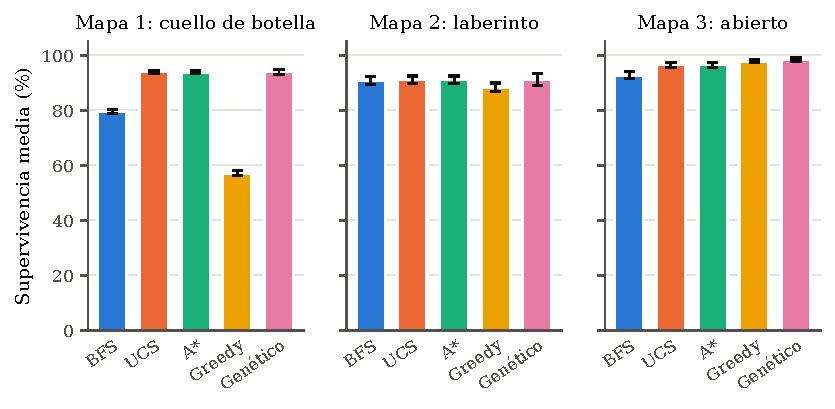
\includegraphics[width=\textwidth]{figuras/supervivencia.pdf}
\caption{Tasa de supervivencia media por mapa y algoritmo. Las barras de error indican el intervalo de confianza del 95\,\% de la media.}
\label{fig:supervivencia}
\end{figure}

\begin{figure}[H]
\centering
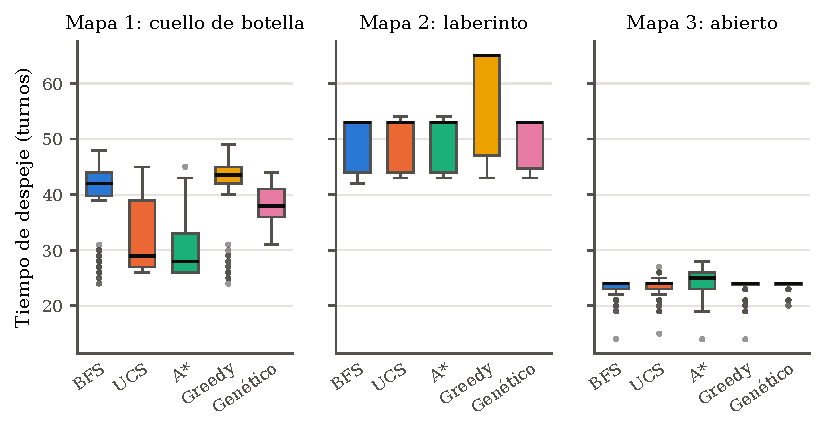
\includegraphics[width=\textwidth]{figuras/tiempo_despeje.pdf}
\caption{Distribución del tiempo de despeje (turnos hasta que evacúa el último sobreviviente) por mapa y algoritmo.}
\label{fig:despeje}
\end{figure}

\subsection{Mapa 1: cuello de botella}

Este mapa es donde más se separan los algoritmos (Figura~\ref{fig:supervivencia}).

\begin{itemize}
    \item \textbf{UCS y A* frente a BFS.} UCS y A* consideran la congestión en el costo y alcanzan una supervivencia cercana al 94\,\%, contra 79.6\,\% de BFS. También despejan el edificio unos 7 a 9 turnos antes (30.2 turnos A* y 32.4 UCS, contra 39.4 BFS).
    \begin{itemize}
        \item BFS minimiza el número de pasos, así que envía a casi todos los agentes por el pasillo central, que es el más corto.
        \item Ese pasillo tiene capacidad para una persona por celda, y la fila avanza a un ritmo de una persona por turno mientras el fuego se acerca.
        \item UCS y A* reparten a los agentes entre los tres pasillos, porque el costo penalizado hace más atractivos los laterales cuando el central se satura.
    \end{itemize}
    Esta comparación muestra directamente el efecto de modelar la congestión.
    \item \textbf{Greedy.} Tiene el peor desempeño: 57.2\,\% de supervivencia y 42.1 turnos. Como su prioridad es solo la distancia Manhattan a la salida, no considera ni el costo acumulado ni la ocupación. Todos los agentes eligen la ruta geométricamente más directa, y el embotellamiento es todavía más severo que con BFS.
    \item \textbf{Algoritmo genético.} En supervivencia iguala a A* (94.0\,\%). Comparando semilla por semilla sobre las 80 comunes, salva a más personas que A* en 27 casos, a menos en 26 y empata en 27, así que no hay una ventaja clara. Tarda más en despejar el edificio (38.1 turnos), porque los retardos de salida que optimiza ordenan el flujo a costa de alargar la evacuación. A cambio, su variabilidad es la menor de todos los algoritmos (desviación de 3.2 turnos).
\end{itemize}

\subsection{Mapa 2: laberinto corporativo}

\begin{itemize}
    \item \textbf{Rendimiento parejo.} Salvo Greedy, todos los algoritmos rinden prácticamente igual: cerca de 91\,\% de supervivencia y 49 turnos. En el laberinto cada sala tiene muy pocas salidas alternativas, así que modelar la congestión no cambia las rutas elegidas.
    \item \textbf{Greedy.} Vuelve a ser el más lento (56.5 turnos, con la mayor dispersión: 8.9 turnos). La distancia Manhattan ignora los muros y lo lleva a pasillos que se acercan a la salida en línea recta pero terminan en callejones sin salida.
    \item \textbf{Distribución bimodal del despeje} (Figura~\ref{fig:despeje}). Se concentra en torno a 43--44 turnos o a 53 turnos, según cuál de los dos focos posibles inicia el incendio. El foco pesa más que el algoritmo.
    \item \textbf{Algoritmo genético.} No logró mejorar su solución inicial en ninguna de las 80 ejecuciones (Figura~\ref{fig:convergencia}) y obtuvo exactamente el mismo resultado que A* en todas las semillas.
\end{itemize}

\subsection{Mapa 3: dispersión abierta}

\begin{itemize}
    \item \textbf{Supervivencia alta en general.} Supera el 92\,\% en todos los algoritmos, y los tiempos de despeje son muy similares (23 a 24 turnos).
    \item \textbf{El orden de Greedy se invierte.} Aquí Greedy (97.9\,\%) y el algoritmo genético (98.4\,\%) superan a UCS y A* (96.6\,\%). Con espacio abierto y pocos muros, la ruta directa rara vez se satura, así que ignorar la congestión no se castiga. La penalización por ocupación, en cambio, lleva a UCS y A* a desvíos innecesarios; A* es el más lento (24.2 turnos).
    \item \textbf{Algoritmo genético.} Su solución inicial asigna a cada agente la ruta candidata más corta sin retardo, lo que se parece a la estrategia de Greedy. Por eso su rendimiento es similar al de Greedy y supera a A* en 23 de las 80 semillas, sin perder en ninguna.
\end{itemize}

\subsection{Costo computacional}

La Figura~\ref{fig:expandidos} muestra los nodos expandidos por simulación, sumando todas las replanificaciones.

\begin{figure}[H]
\centering
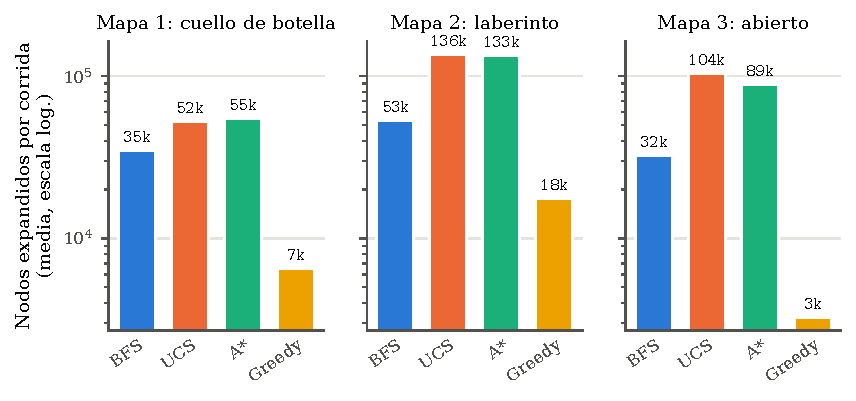
\includegraphics[width=\textwidth]{figuras/nodos_expandidos.pdf}
\caption{Nodos expandidos por simulación (media, escala logarítmica), sumando todas las replanificaciones. No incluye el algoritmo genético, cuyo costo está en las simulaciones de evaluación de aptitud.}
\label{fig:expandidos}
\end{figure}

\begin{itemize}
    \item \textbf{Greedy} es por lejos el más barato (entre 3\,300 y 17\,500 nodos), porque avanza directamente hacia la salida.
    \item \textbf{BFS} expande entre 32\,000 y 53\,000 nodos.
    \item \textbf{UCS y A*} son los más costosos (entre 52\,000 y 136\,000 nodos), porque además de expandir por costo acumulado replanifican cada vez que el fuego avanza o un agente queda bloqueado.
    \item \textbf{A* casi no ahorra frente a UCS}; solo en el Mapa 3 expande un 15\,\% menos. Las penalizaciones por congestión y por cercanía al fuego son grandes comparadas con la distancia Manhattan, que en consecuencia orienta poco la búsqueda. Además, la implementación utilizada no descarta los nodos repetidos de la cola de prioridad y vuelve a expandirlos.
\end{itemize}

\subsection{Convergencia del algoritmo genético}

\begin{figure}[H]
\centering
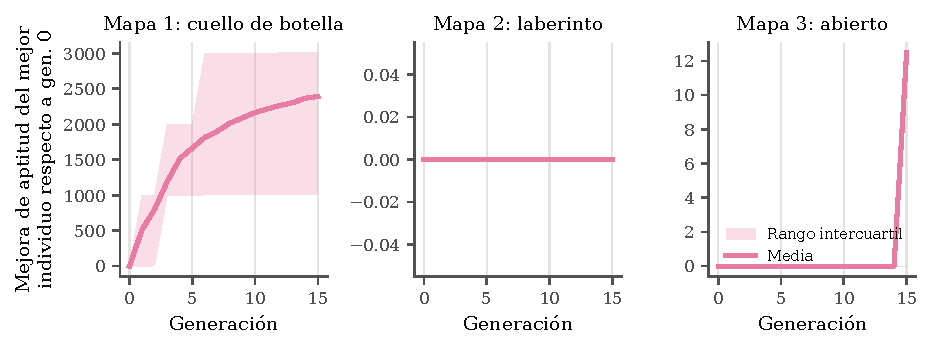
\includegraphics[width=\textwidth]{figuras/convergencia_genetico.pdf}
\caption{Convergencia del algoritmo genético: mejora de la aptitud del mejor individuo respecto a la generación inicial (media y rango intercuartil de las 80 ejecuciones).}
\label{fig:convergencia}
\end{figure}

En el Mapa 1 el algoritmo genético mejoró su solución inicial en las 80 ejecuciones, con una mejora media de unos 2\,400 puntos de aptitud, equivalente a salvar a unas 2 personas más por escenario evaluado. En el Mapa 2 no mejoró en ninguna ejecución, y en el Mapa 3 solo en una. En esos dos mapas la solución inicial (todos por su ruta más corta y sin retardo) ya era la mejor que encontró la búsqueda.

\section{Conclusiones}

\begin{itemize}
    \item \textbf{Modelar la congestión importa donde hay cuellos de botella.} En el Mapa 1, UCS y A* salvan a unas 5 personas más por simulación que BFS (14.5 puntos de supervivencia sobre 34 agentes).
    \item \textbf{La heurística sola es riesgosa.} Greedy es el más eficiente computacionalmente y funciona bien en espacios abiertos, pero concentra a los agentes y colapsa en el cuello de botella.
    \item \textbf{El algoritmo genético nunca fue peor que la mejor búsqueda en supervivencia}, pero solo mejoró su solución inicial en el Mapa 1, y con un costo computacional muy superior.
    \item \textbf{Limitación.} Los parámetros del algoritmo genético (20 individuos, 15 generaciones) están limitados por el tiempo de ejecución. Con más población y más generaciones es posible que mejore también en los otros mapas.
\end{itemize}

\section*{Uso de código de terceros e IA generativa}

Las funciones de búsqueda (\texttt{breadth\_first\_search}, \texttt{dijkstra\_search}, \texttt{a\_star\_search}, \texttt{greedy\_best\_first\_search} y sus estructuras auxiliares) fueron tomadas de Red Blob Games \cite{redblob-impl,redblob-intro}, bajo licencia Apache 2.0, sin modificar su lógica. El entorno, la simulación, el algoritmo genético y los scripts de benchmark son implementación propia, desarrollada con asistencia de Claude (Anthropic), modelo Claude Opus 5.5. El detalle está en \texttt{REFERENCIAS.md}.

\begin{thebibliography}{9}
\bibitem{redblob-impl}
A.~Patel, \emph{Implementation of A*}, Red Blob Games, 2014 (rev. 2026). Código fuente: \url{https://www.redblobgames.com/pathfinding/a-star/implementation.py}. Licencia Apache 2.0. Consultado el 28-09-2026.

\bibitem{redblob-intro}
A.~Patel, \emph{Introduction to the A* Algorithm}, Red Blob Games. \url{https://www.redblobgames.com/pathfinding/a-star/introduction.html}. Consultado el 28-09-2026.
\end{thebibliography}

\end{document}
